\PassOptionsToPackage{unicode,pdfusetitle}{hyperref}
\PassOptionsToPackage{hyphens}{url}
\PassOptionsToPackage{dvipsnames,svgnames,x11names}{xcolor}

\documentclass[10pt]{beamer}

\usetheme{moloch}
\usefonttheme{professionalfonts}
\setbeamertemplate{page number in head/foot}[appendixframenumber]

\usepackage[T1]{fontenc}
\usepackage{lmodern}
\usepackage{bm}
\usepackage{amssymb,amsmath,mathtools,amsthm}
\usepackage{textcomp}
\usepackage{pifont}
\usepackage{dirtree}
\usepackage{siunitx}

\usepackage{upquote} % straight quotes in verbatim environments
\usepackage{microtype}
\UseMicrotypeSet[protrusion]{basicmath} % disable protrusion for tt fonts

\usepackage{xmpmulti}

% listings
\usepackage{listings}

% Define a custom color
\definecolor{backcolour}{rgb}{0.95,0.95,0.95}
\definecolor{codegreen}{rgb}{0,0.6,0}
\definecolor{mygray}{rgb}{0.6,0.6,0.6}

\lstdefinestyle{myStyle}{
  backgroundcolor=\color{backcolour},
  frame=single,
  % commentstyle=\color{codegreen},
  basicstyle=\ttfamily,
  breakatwhitespace=false,
  breaklines=true,
  keepspaces=true,
  numbers=left,
  % numbersep=5pt,
  numberstyle=\footnotesize\color{mygray},
  showspaces=false,
  showstringspaces=false,
  showtabs=false,
  tabsize=2,
}

% Use \lstset to make myStyle the global default
\lstset{style=myStyle}

\usepackage{xcolor}
\usepackage{xurl} % add URL line breaks if available
\usepackage{bookmark}

\usepackage[noabbrev,nameinlink]{cleveref}

\usepackage{hyperref}

\hypersetup{%
  colorlinks = true,
  linkcolor  = mLightGreen,
  filecolor  = mLightGreen,
  citecolor  = mLightGreen,
  urlcolor   = mLightGreen
}

% subfigures
\usepackage{subcaption}

% algorithms
\usepackage[ruled,vlined]{algorithm2e}
\resetcounteronoverlays{algocf}

% tikz and pgfplots stuff
\usepackage{tikz}
\usetikzlibrary{arrows,shapes,positioning,intersections}
\usepackage{pgfplots}
\usepgfplotslibrary{external,colormaps}
\pgfplotsset{compat=1.15}
%\tikzexternalize

% \definecolor{graphicbackground}{rgb}{0.96,0.96,0.8}
% \setbeamercolor{background canvas}{bg=graphicbackground}

\usepackage{booktabs}

\date{June 28, 2024}
\titlegraphic{
\includegraphics{figures/logo.pdf}}

% bibliography
\usepackage[style=authoryear,url=false,backend=biber]{biblatex}
\addbibresource{bibliography.bib}

% title block
\title{Optimization and Algorithms in Sparse Regression}
\subtitle{Screening Rules, Coordinate Descent, and Normalization}
\author{Johan Larsson}
\institute{Department of Statistics, Lund University}


% operators
\DeclareMathOperator*{\argmax}{arg\,max}
\DeclareMathOperator*{\argmin}{arg\,min}
\DeclareMathOperator{\E}{\text{E}}
\DeclareMathOperator{\var}{var}
\DeclareMathOperator{\cov}{cov}
\DeclareMathOperator{\sign}{sign}
\DeclareMathOperator{\card}{card}
\DeclareMathOperator{\cumsum}{cumsum}
\DeclareMathOperator*{\prox}{prox}

% macros
\newcommand{\pkg}[1]{\textsf{#1}}
\renewcommand{\vec}{\vectorsym}
\newcommand{\mat}{\matrixsym}
\newcommand{\du}{\mathrm{d}}

\makeatletter
\newcommand\notsotiny{\@setfontsize\notsotiny\@vipt\@viipt}
\makeatother



\begin{document}

\maketitle

% \begin{frame}[c]
%   \frametitle{Overview}
%
%   \tableofcontents
% \end{frame}

\begin{frame}[c]
  \frametitle{Synopsis}

  \begin{exampleblock}{Overarching Theme}
    Practical concerns in sparse regression: speed, accuracy, and reproducibility.
  \end{exampleblock}

  \pause

  \begin{block}{Overview}
    \begin{description}[I--III]
      \item[I--III] Screening rules
      \item[IV] Benchmarking optimization methods
      \item[V] Coordinate descent (an optimization method) for SLOPE
      \item[VI] Normalization and regularization
    \end{description}
  \end{block}
\end{frame}

\section{The Strong Screening Rule for SLOPE (Paper I)}

\begin{frame}[c]
  \frametitle{The Strong Screening Rule for SLOPE}

  Published and presented at NeurIPS 2020\footnote{\fullcite{larsson2020b}}

  \bigskip

  Co-written with supervisors Małgorzata Bogdan and Jonas Wallin.

  \begin{center}
    \hfill%
    \frame{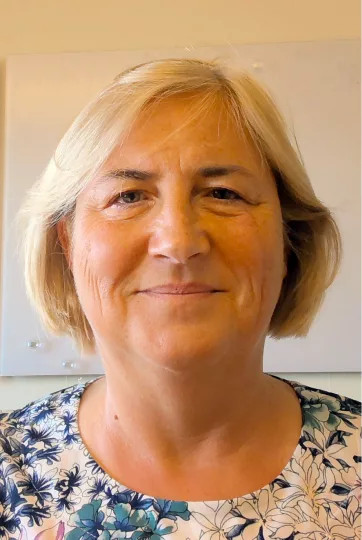
\includegraphics[height=3cm]{figures/gosia.jpeg}}\hfill%
    \frame{
\includegraphics[height=3cm]{figures/jonas.jpg}}\hfill\null
  \end{center}

\end{frame}

\begin{frame}[c]
  \frametitle{Motivation}

  \begin{itemize}[<+->]
    \item Data sets are growing in size.
    \item Fitting models to sets of millions (maybe billions) of features is computationally costly.
    \item Hyperparameter tuning increases costs further.
  \end{itemize}

\end{frame}

\begin{frame}[c]
  \frametitle{Screening Rules}

  \begin{block}{Basic Insight}
    \begin{itemize}
      \item The support set is small in sparse regression, especially when \(p \gg n\).\footnote{The
              lasso can for instance at most select \(\min(n, p)\) features.}
      \item Can we somehow figure this support \textbf{before} fitting the model?
    \end{itemize}
  \end{block}

  \pause

  \begin{block}{General Idea}
    \begin{enumerate}
      \item Estimate how likely it is that a feature is in the support set.
      \item If unlikely, discard it.
      \item Fit a reduced model.
      \item If we were wrong, just refit the model with missing features added.
    \end{enumerate}
  \end{block}

  \medskip\pause

  Turns out to be a pretty good idea!
\end{frame}

\begin{frame}[c]
  \frametitle{Optimality Conditions and the Gradient}

  \begin{columns}[T]
    \begin{column}{0.51\textwidth}
      \begin{block}{Optimality Condition}
        \(\bm{\beta}\) is optimal if
        \begin{equation*}
          \boldsymbol{0} \in \nabla g(\bm{\beta}) + \partial h(\vec{\beta}),
        \end{equation*}
        where \(\partial h (\vec{\beta})\) is the subdifferential of the penalty term \(h\).
      \end{block}

      \pause

      \begin{block}{The Lasso}
        Here we have
        \[
          \partial h (\beta)_j =
          \begin{cases}
            \{
            \lambda\sign(\beta_j)\} & \text{if } \beta_j \neq 0, \\
            [-\lambda, \lambda]     & \text{if } \beta_j = 0.
          \end{cases}
        \]
        If \(|\nabla g(\vec{\beta}^*)_j| < \lambda,\) \alert{then \(\beta_j^* = 0\)}.
      \end{block}

    \end{column}
    \begin{column}{0.39\textwidth}

      \begin{figure}[htpb]
        \centering
        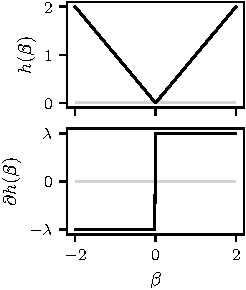
\includegraphics{figures/paper1-subgradient-split.pdf}
        \caption{%
          The lasso penalty \(h(\bm{\beta}) = \lambda \lVert \bm{\beta}\rVert_1\) and its subdifferential at \(\lambda = 1\).
        }
      \end{figure}
    \end{column}
  \end{columns}

\end{frame}

\begin{frame}[c]
  \frametitle{The Lasso Path}
  \begin{figure}[htpb]
    \centering
    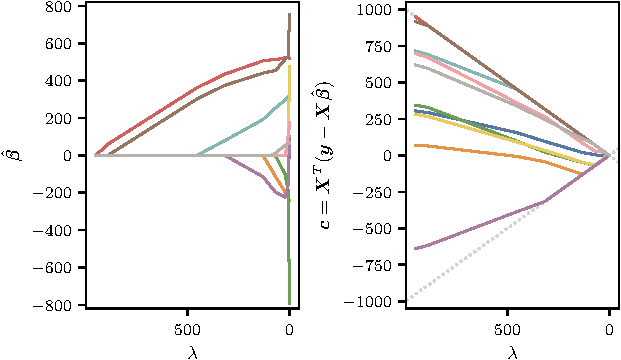
\includegraphics[]{figures/paper1-cor-coef-lasso-path.pdf}
    \caption{%
      Coefficients and correlations (\(\bm{c}\)) along the lasso path
    }
  \end{figure}
\end{frame}

\begin{frame}[c]
  \frametitle{Strong Rule for the Lasso}

  \begin{figure}[htpb]
    \centering
    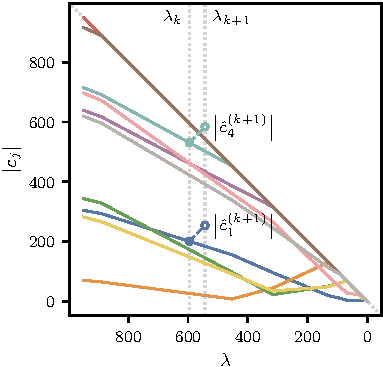
\includegraphics[]{figures/paper1-strong-rule.pdf}
    \caption{%
    The strong rule for the lasso~\parencite{tibshirani2012}. \(|\hat{c}_j^{(k+1)}| = |c_j^{(k)}| + \lambda_{k} - \lambda_{k+1} \) is the absolute correlation estimate for feature \(j\) at step \(k+1\).
    }
  \end{figure}
\end{frame}

\begin{frame}[c]
  \frametitle{Strong Rule for SLOPE}

  Same idea as for lasso strong rule! Just need the subdifferential.

  % TODO: give an example

  \begin{block}{SLOPE Subdifferential}

    The set of all \(\bm{g} \in \mathbb{R}^p\) such that
    \[
      \small
      \vec{g}_{\mathcal{A}_i} =
      \left\{\vec{s} \in \mathbb{R}^{|{\mathcal{A}_i}|} \bigm\vert
        \begin{cases}
          \mathop{\mathrm{cumsum}}(|\bm{s}|_\downarrow - \bm{\lambda}_{R(\bm{s})_{\mathcal{A}_i}}) \preceq \mathbf{0} & \text{if } \beta_{\mathcal{A}_i} = \mathbf{0}, \\
          \mathop{\mathrm{cumsum}}(|\bm{s}|_\downarrow - \bm{\lambda}_{R(\bm{s})_{\mathcal{A}_i}}) \preceq \mathbf{0}                                                  \\
          \quad\,\text{and } \sign(\bm{\beta}_{\mathcal{A}_i}) = \sign(\bm{s})                                                                                         \\
          \quad\,\text{and } \sum_{j \in \mathcal{A}_i}\left(|s_j| - \lambda_{R(\bm{s})_j}\right) = 0                 & \text{otherwise.}
        \end{cases}
      \right\}
    \]
  \end{block}

  \medskip

  \begin{itemize}
    \item \(\mathcal{A}_i\) defines a \alert{cluster} containing indices of coefficients
          equal in absolute value.
    \item \(R(\bm{x})\) returns \alert{ranks} of absolute values of elements in \(\bm{x}\).
    \item \(|\vec{x}|_\downarrow\) returns the absolute values of \(x\) sorted in non-increasing
          order.
  \end{itemize}

\end{frame}

\begin{frame}[c]
  \frametitle{Results: Effectiveness}

  \begin{figure}[htpb]
    \centering
    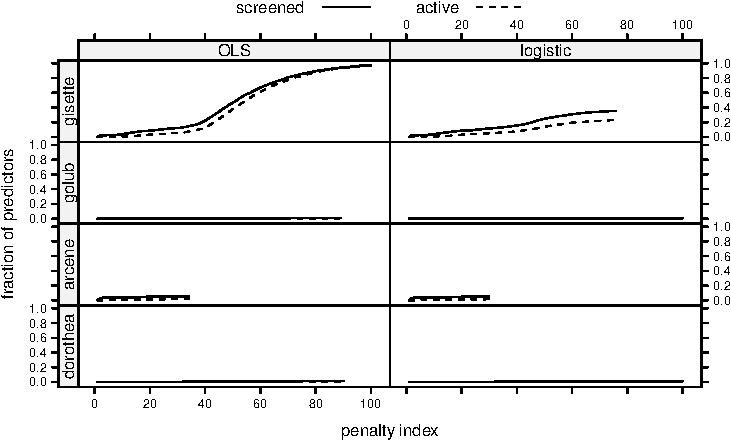
\includegraphics[width=\textwidth]{figures/paper1-efficiency-real.pdf}
    \caption{%
      Effectiveness for some real data sets
    }
  \end{figure}
\end{frame}

\begin{frame}[c]
  \frametitle{Results: Speed}
  \begin{table}
    \caption{Time to fit lasso paths using either the strong screening rule or no rule.}
    \centering
    \small
    \begin{tabular}{llS[table-format=4.0]S[table-format=6.0]S[table-format=5.0]S[table-format=4.0]}
      \toprule
      \multicolumn{1}{c}{} & \multicolumn{1}{c}{} & \multicolumn{1}{c}{} & \multicolumn{1}{c}{} & \multicolumn{2}{c}{{Time (s)}}               \\
      \cmidrule(l{3pt}r{3pt}){5-6}
      Dataset              & Model                & $n$                  & $p$                  & {No Screening}                 & {Screening} \\
      \midrule
      dorothea             & Logistic             & 800                  & 88119                & 914                            & 14          \\
      e2006-tfidf          & Least squares        & 3308                 & 150358               & 43353                          & 4944        \\
      news20               & Multinomial          & 1000                 & 62061                & 5485                           & 517         \\
      physician            & Poisson              & 4406                 & 25                   & 34                             & 34          \\
      \bottomrule
    \end{tabular}
  \end{table}
\end{frame}

% \begin{frame}[c]
%   \frametitle{Heuristic Screening and Violations}
%
%   \begin{itemize}
%     \item The rule is \textbf{heuristic}\footnote{As opposed to \emph{safe}.}, which means that
%           \alert{violations} may occur.
%     \item But they are so rare and checking for and refitting with them so cheap that it rarely
%           matters.
%   \end{itemize}
%
%   \pause
%
%   \begin{figure}[htpb]
%     \centering
%     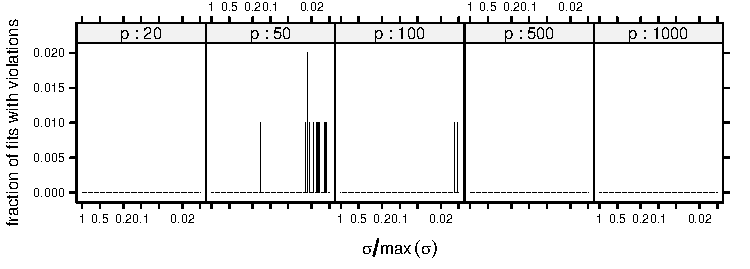
\includegraphics[width=\textwidth]{figures/paper1-violations.pdf}
%     \caption{%
%       Violations of the strong rule for SLOPE
%     }
%   \end{figure}
%
% \end{frame}

\begin{frame}[c]
  \frametitle{Summary}

  \begin{exampleblock}{Contributions}
    \begin{itemize}
      \item The first screening rule for SLOPE
      \item A new formulation of the subdifferential for SLOPE
      \item Implementation in the R package
            \texttt{SLOPE}\footnote{\url{https://doi.org/10.32614/CRAN.package.SLOPE}}
    \end{itemize}
  \end{exampleblock}

  \pause

  \begin{alertblock}{Limitations}
    \begin{itemize}
      \item Somewhat conservative
      \item Heuristic\footnote[frame]{As opposed to \emph{safe}.} rule, so violations may occur. But
            are not problematic in practice.
    \end{itemize}
  \end{alertblock}
\end{frame}

\section{Look-Ahead Screening Rules for the Lasso (Paper II)}

\begin{frame}[c]
  \frametitle{Look-Ahead Screening Rules for the Lasso}
  Published in EYSM 2021\footnote{\fullcite{larsson2021}}

  \bigskip

  \begin{center}
    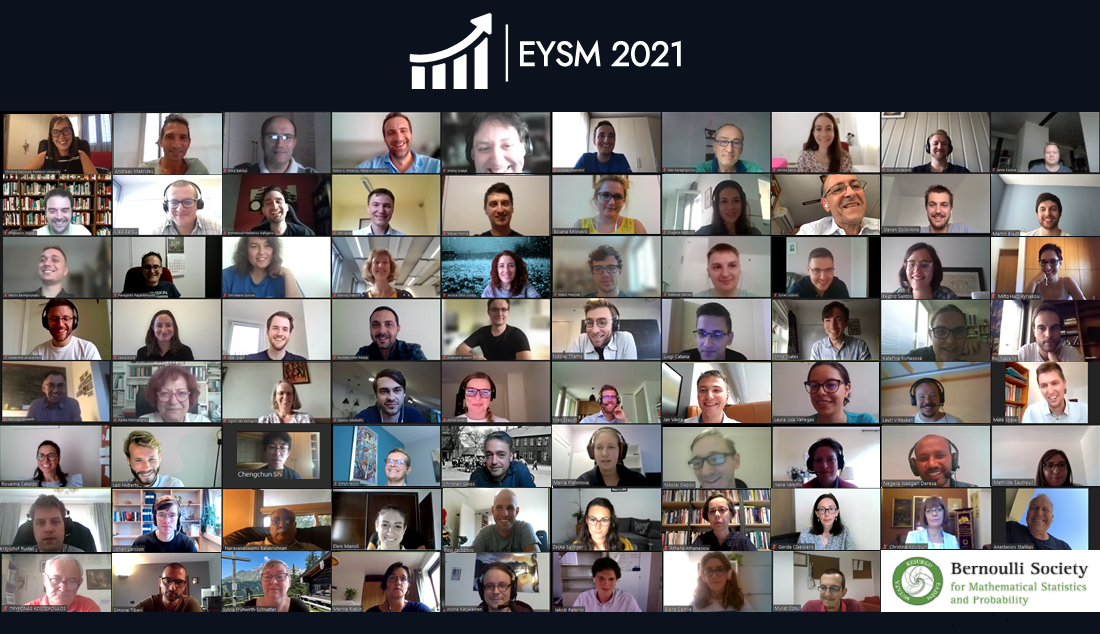
\includegraphics[height=4cm]{figures/eysm.png}
  \end{center}

\end{frame}

\begin{frame}[c]
  \frametitle{Motivation}
  \begin{itemize}[<+->]
    \item Even if screening rules improve the speed remarkably, they still involve costs (e.g.
          gradient computations).
    \item Previous screening rules just look one-step ahead.
    \item But information from the current step is useful for more than the next one, so why not look
          further ahead?
  \end{itemize}
\end{frame}

\begin{frame}[c]
  \frametitle{Gap Safe Screening}

  Gap Safe screening~\parencite{fercoq2015} uses the \textbf{duality gap} as a basis for a
  safe screening rule, and discards the \(j\)th predictor if
  \begin{equation}
    \label{eq:gap-safe}
    |\vec{x}_j^\intercal \vec{\theta}_\lambda| + \lVert \vec{x}_j\rVert_2
    \sqrt{
      \frac{1}{\lambda_+^2}
      \big(\mathcal{P}(\vec{\beta}_\lambda; \lambda_+) -
      \mathcal{D}(\vec{\theta}_\lambda; \lambda_+)\big)
    }
    < 1
  \end{equation}\pause
  where \(\vec{\theta}_\lambda\) is the \alert{scaled} dual variable,
  \[
    \bm{\theta}_\lambda = \frac{\vec{y} - \bm{X\beta}_\lambda}{
      \max\big( \lVert \bm{X}^\intercal(\bm{y} - \bm{X\beta}_\lambda)\rVert_\infty, \lambda\big)}.
  \]
  \pause\medskip

  \Cref{eq:gap-safe} is \alert{quadratic} in \(\lambda\),
  so we can use it to find the next critical value for \(\lambda\) and
  screen for \alert{all} steps ahead.

\end{frame}

\begin{frame}[c]
  \frametitle{Simple Example}

  \begin{figure}[htpb]
    \centering
    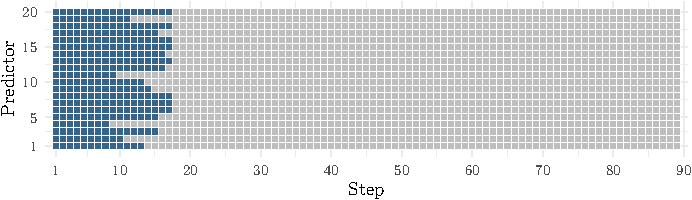
\includegraphics[width=\textwidth]{figures/paper2-casestudy.pdf}
    \caption{%
      The lasso path for a sample of 20 features from the leukemia data set. The squares
      show for which steps the feature can be discarded.
    }
  \end{figure}
\end{frame}

\begin{frame}[c]
  \frametitle{Benchmarks}

  \begin{figure}[htpb]
    \centering
    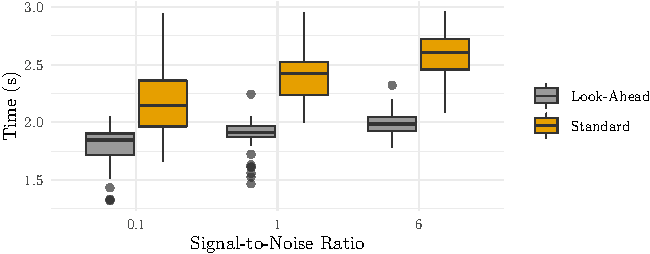
\includegraphics[width=\textwidth]{figures/paper2-simulated-data.pdf}
    \caption{%
      Benchmarks of time to fit the full lasso path with or without look-ahead screening.
    }
  \end{figure}
\end{frame}

\begin{frame}[c]
  \frametitle{Summary}
  \begin{exampleblock}{Contributions}
    \begin{itemize}
      \item Simple, safe, and essentially free screening rule for the lasso (and related problems)
      \item Moderate improvements in speed
    \end{itemize}
  \end{exampleblock}

  \pause

  \begin{alertblock}{Limitations}
    \begin{itemize}
      \item Needs a safe rule
    \end{itemize}
  \end{alertblock}
\end{frame}

\section{The Hessian Screening Rule (Paper~III)}

\begin{frame}[c]
  \frametitle{The Hessian Screening Rule}

  \begin{columns}
    \begin{column}{0.45\textwidth}

      Published and presented at NeurIPS 2022\footnote[frame]{\fullcite{larsson2022b}}

      \bigskip

      Co-authored with Jonas
    \end{column}
    \begin{column}{0.45\textwidth}
      
\includegraphics[width=\textwidth]{figures/neurips.pdf}
    \end{column}
  \end{columns}
\end{frame}

\begin{frame}[c]
  \frametitle{Motivation}

  \begin{itemize}
    \item Previous screening rules, like the strong rule, struggle with highly correlated features.
    \item Previous rules do not use information about the correlations along the lasso path.
  \end{itemize}
\end{frame}

% \begin{frame}
%   \frametitle{Screening Rules Seen As Gradient Estimates}
%
%   Recall that \(\vec{c} = -\nabla g(\vec{\beta})\) and hence optimality condition is
%   \(\vec{c} \in \partial h (\vec{\beta})\).
%
%   \medskip
%
%   \begin{exampleblock}{Lasso Screening Rule Template }
%     \begin{enumerate}
%       \item Replace \(\vec{c}\) with an estimate \(\tilde{\vec{c}}\).
%       \item If \(|\tilde{\vec{c}}_j| < \lambda\), discard feature \(j\).
%     \end{enumerate}
%
%     \medskip
%
%     If \(\tilde{\vec{c}}\) is accurate and not too conservative, we have a useful rule.
%   \end{exampleblock}
% \end{frame}

\begin{frame}
  \frametitle{The Hessian Screening Rule}
  \begin{columns}
    \begin{column}{0.45\textwidth}
      For the ordinary lasso,
      \begin{align*}
        g(\bm{\beta})        & = \frac 1 2 \lVert \vec{y} - \bm{X \beta} \rVert_2^2, \\
        \nabla g(\bm{\beta}) & = \bm{X}^\intercal(\bm{X\beta} - \bm{y}),
      \end{align*}
      solution is \alert{piecewise linear}.
    \end{column}
    \begin{column}{0.45\textwidth}
      \centering
      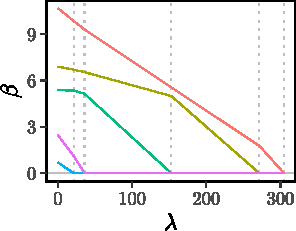
\includegraphics[width=\textwidth]{figures/paper3-lasso-path.pdf}
    \end{column}
  \end{columns}

  \bigskip\pause

  % It turns out that we can express the solution as a function of \(\lambda\):
  % \begin{equation*}
  %   \hat{\bm{\beta}}(\lambda) = \big({\bm{X}_\mathcal{A}}^\intercal \bm{X}_\mathcal{A}\big)^{-1}
  %   \big({\bm{X}_\mathcal{A}}^\intercal \bm{y} - \lambda \sign(\hat{\bm{\beta}}_\mathcal{A})\big).
  % \end{equation*}
  %
  % \pause

  If active set is constant in \([\lambda_k,\lambda_{k+1}]\), we can express the solution as
  \begin{equation*}
    \hat{\vec{\beta}}(\lambda_{k+1})_\mathcal{A} =
    \hat{\vec{\beta}}(\lambda_k)_\mathcal{A} -
    (\lambda_k - \lambda_{k+1})\big({\bm{X}_\mathcal{A}}^\intercal \bm{X}_\mathcal{A}\big)^{-1}
    \sign\big(\hat{\vec{\beta}}(\lambda_k)_\mathcal{A}\big).
  \end{equation*}

  \pause

  \begin{exampleblock}{Hessian Screening Rule (Basic Form)}
    Plug \(\hat{\bm{\beta}}\) into the gradient at step \(k + 1\):
    \begin{equation*}
      \begin{aligned}
        \tilde{\bm{c}}^H(\lambda_{k+1})
         & = -\nabla g\big(\hat{\vec{\beta}}(\lambda_{k+1})_\mathcal{A}\big)                      \\
         & = \bm{c}(\lambda_k) + (\lambda_{k+1} - \lambda_k)\bm{X}^\intercal {\bm{X}_\mathcal{A}}
        \big({\bm{X}_\mathcal{A}}^\intercal \bm{X}_\mathcal{A}\big)^{-1}
        \sign\big(\hat{\vec{\beta}}(\lambda_k)_\mathcal{A}\big).
      \end{aligned}
    \end{equation*}
  \end{exampleblock}

\end{frame}

\begin{frame}[c]
  \frametitle{Screening Rule Comparison}

  \begin{figure}[tpb]
    \centering
    \pgfplotsset{width=9cm,height=7cm}
    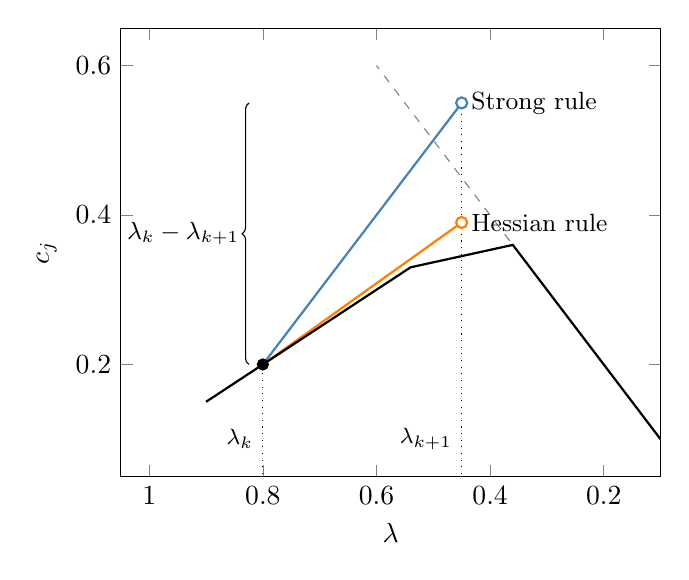
\begin{tikzpicture}
  \begin{axis}[
      ylabel = \(c_j\),
      xlabel = \(\lambda\),
      xmin = 0.1,
      xmax = 1.05,
      ymin = 0.05,
      ymax = 0.65,
      max space between ticks = 1000pt,
      try min ticks = 5,
      x dir = reverse
    ]
    \addplot[style = dashed, color=Grey]
    coordinates {
        (0.1,0.1)
        (0.6,0.6)
      };
    \addplot[thick,color=SteelBlue]
    coordinates {
        (0.8,0.2)
        (0.45,0.55)
      };
    \addplot[thick,color=orange]
    coordinates {
        (0.8,0.2)
        (0.45,0.39)
      };
    \addplot[thick]
    coordinates {
        (0.9,0.15)
        (0.54,0.33)
        (0.36,0.36)
        (0.1,0.1)
      };
    \draw [decorate,decoration={brace},xshift=-5pt]
    (0.8,0.2) -- (0.8,0.55)node [left,black,midway] {\small
      \(\lambda_{k}-\lambda_{k + 1}\)};

    \node [right] at (0.45, 0.39) {\small Hessian rule};
    \addplot[thick,mark=*,color=orange,fill=white] coordinates {(0.45,0.39)};

    \node [right] at (0.45, 0.55) {\small Strong rule};
    \addplot[thick,mark=*,color=SteelBlue,fill=white] coordinates {(0.45,0.55)};

    \addplot[mark=*] coordinates {(0.8,0.2)};

    \addplot[style=dotted]
    coordinates {
        (0.45,0.0)
        (0.45,0.55)
      };
    \addplot[style=dotted]
    coordinates {
        (0.8,0.0)
        (0.8,0.2)
      };
    \node [left] at (0.45,0.1) {\footnotesize\(\lambda_{k + 1}\)};
    \node [left] at (0.8,0.1) {\footnotesize\(\lambda_{k}\)};
  \end{axis}
\end{tikzpicture}

    \caption{%
      The strong and Hessian screening rules in action
    }
  \end{figure}
\end{frame}

\begin{frame}{Results: Effectiveness}
  \begin{figure}
    \centering
    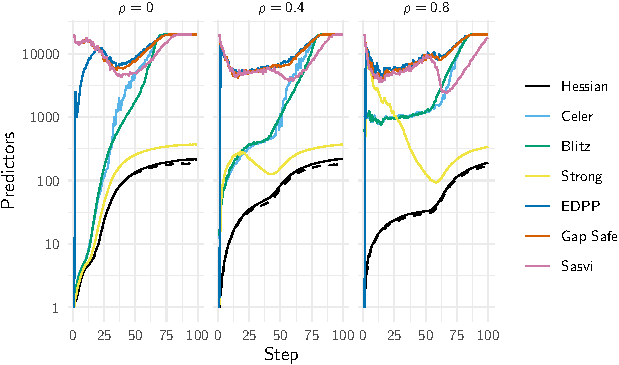
\includegraphics[width=\textwidth]{figures/paper3-simulateddata-efficiency}
    \caption{%
      Features screened for a lasso path for \(\ell_1\)-regularized
      least-squares to a design with varying correlation (\(\rho\)), \(n = 200\), and \(p =
      \num{20000}\).
    }
  \end{figure}
\end{frame}

\begin{frame}{Results: Simulated Data}
  \begin{figure}
    \centering
    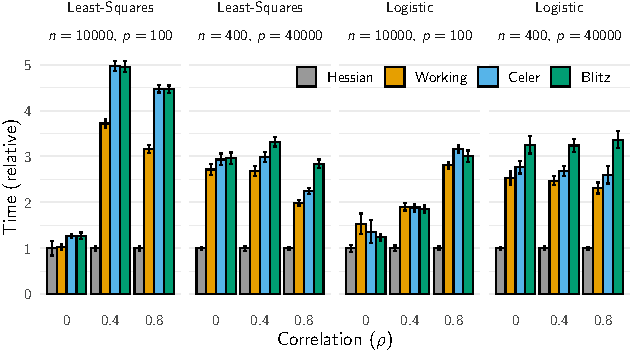
\includegraphics{figures/paper3-simulateddata-timings}
    \caption{
      Time to fit a full path of \(\ell_1\)-regularized least-squares and
      logistic regression to a design with \(n\) observations, \(p\) features, and pairwise
      correlation between features of \(\rho\).
    }
  \end{figure}
\end{frame}

\begin{frame}[c]
  \frametitle{Summary}
  \begin{exampleblock}{Contributions}
    \begin{itemize}
      \item New screening rule that performs better in general and particularly for highly correlated
            features
      \item Provides better warm starts along the path
      \item Works well for both least-squares and logistic regression
            % \item Can be used in combination with approximate homotopy
    \end{itemize}
  \end{exampleblock}

  \pause
  \begin{alertblock}{Limitations}
    \begin{itemize}
      \item Not optimal for problems with more complex Hessians
      \item Implementation is a bit more involved.
            % \item Although the rule works well with high correlation, speed-ups are not commensurate since
            %       our warm starts are worse.
    \end{itemize}
  \end{alertblock}
\end{frame}

\section{Benchopt: Reproducible, Efficient and Collaborative Optimization Benchmarks (Paper~IV)}

\begin{frame}[c]
  \frametitle{Benchopt}

  \begin{columns}
    \begin{column}{0.45\textwidth}
      Published and presented at NeurIPS 2022\footnote[frame]{\fullcite{moreau2022a}}

      \medskip

      Too many authors (20) to list here!
    \end{column}
    \begin{column}{0.45\textwidth}
      
\includegraphics[width=\textwidth]{figures/paper4-benchopt_logo.pdf}
    \end{column}
  \end{columns}
\end{frame}

\begin{frame}
  \frametitle{Motivation}
  \begin{columns}[c]
    \begin{column}{0.45\textwidth}
      \begin{itemize}[<+->]
        \item Surging number of optimization methods
        \item Optimal choice depends on problem
              \begin{itemize}
                \item Data set (dimensions, sparsity, conditioning, normalization)
                \item Hyper-parameters (regularization)
                      % \item Implementation (programming language)
                \item Hardware (GPU acceleration)
              \end{itemize}
        \item Reproducibility
      \end{itemize}
    \end{column}
    \begin{column}{0.45\textwidth}
      \begin{figure}[htpb]
        \centering
        \frame{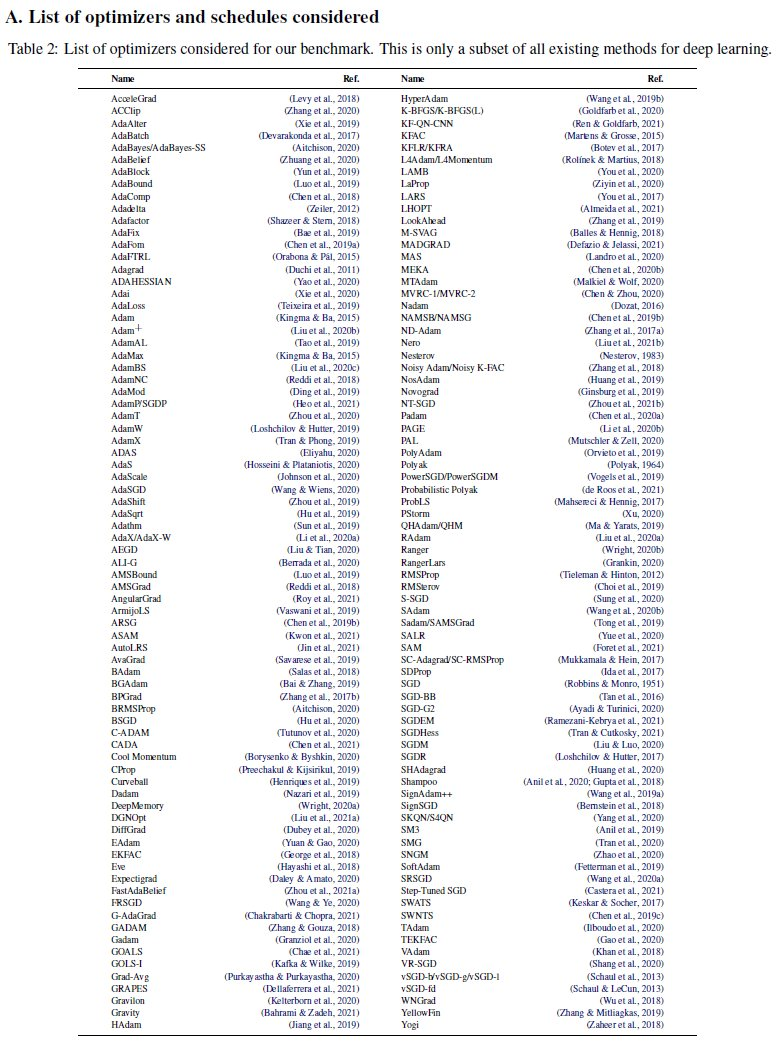
\includegraphics[width=0.91\textwidth]{figures/paper4-DL_optimizers.jpg}}
        \caption{%
          Methods benchmarked in \textcite{schmidt2021}
        }
      \end{figure}

    \end{column}
  \end{columns}
\end{frame}

\begin{frame}[c]
  \frametitle{Benchopt Tries to Solve This!}

  \begin{figure}[htpb]
    \centering
    \multiinclude[format=pdf,start=0,graphics={width=\textwidth}]{figures/paper4-benchopt_schema}
    \caption{%
      Schematic over how benchopt works
    }
  \end{figure}
\end{frame}

\begin{frame}[fragile]
  \frametitle{Example: SLOPE}

  Install benchopt in an isolated environment.
  \begin{lstlisting}[language=bash,basicstyle=\ttfamily\small]
conda create -n benchenv python
conda activate benchenv
pip install -U benchopt
\end{lstlisting}

  \pause\medskip

  Install the benchmark (solvers and data sets).
  \begin{lstlisting}[language=bash,basicstyle=\ttfamily\small]
benchopt install benchmark_slope -s rSLOPE -s PGD
\end{lstlisting}

  \pause\medskip

  And run it!

  \begin{lstlisting}[language=bash,basicstyle=\ttfamily\small]
benchopt run benchmark_slope \
  -o SLOPE[reg=0.5,fit_intercept=False,q=0.1] \
  -s PGD[prox=prox_isotonic] -s rSLOPE \
  -d Simulated[n_features=500,n_samples=200]
\end{lstlisting}

\end{frame}

\begin{frame}[c]
  \begin{figure}[htpb]
    \centering
    \frame{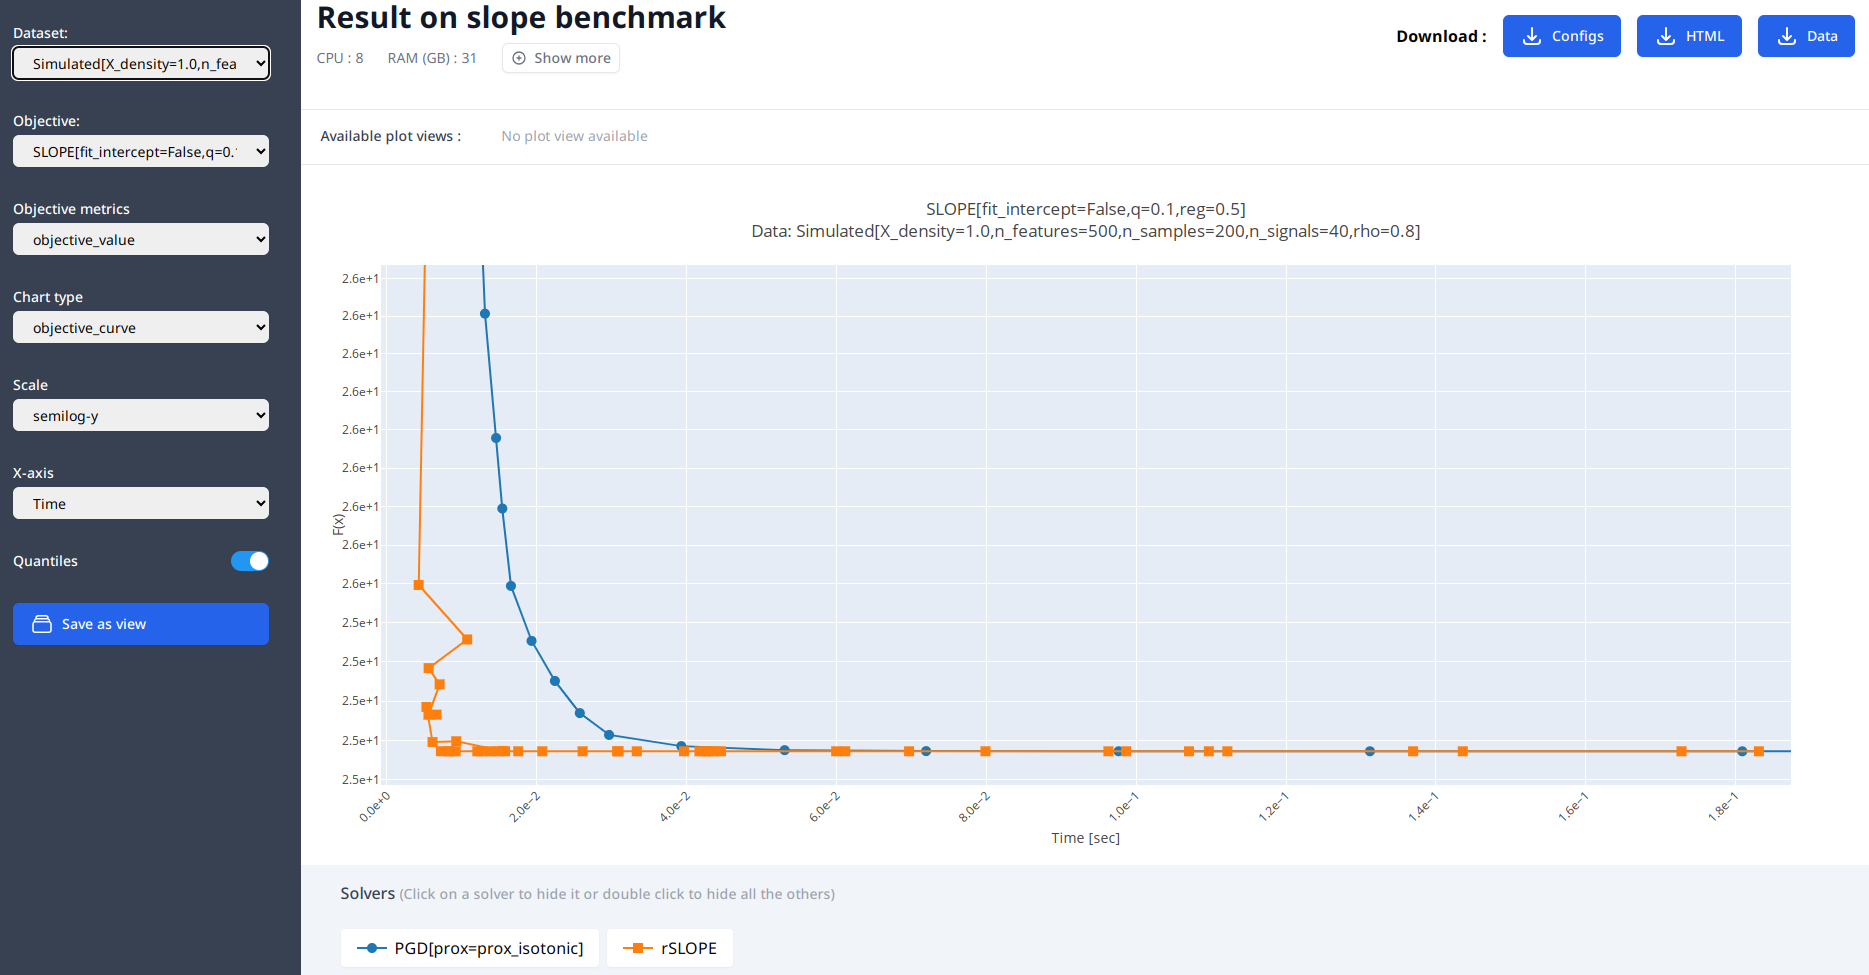
\includegraphics[width=\textwidth]{figures/paper4-benchopt-example.png}}
    \caption{%
      Benchopt benchmark results for SLOPE
    }
  \end{figure}
\end{frame}

% \begin{frame}
%   \frametitle{Publishing Results}
%
%   It is easy to publish benchmark results too!
%
%   \begin{figure}[htpb]
%     \centering
%     \frame{\includegraphics[width=.7\textwidth]{figures/benchopt_results}}
%     \caption{%
%       Results published at \url{https://benchopt.github.io/results/}
%     }
%   \end{figure}
% \end{frame}

\begin{frame}[fragile]
  \frametitle{Benchmark Structure}

  % A benchopt benchmark is a directory with
  % \begin{itemize}
  %   \item an \lstinline+objective.py+ file with an \lstinline+Objective+,
  %   \item a directory \lstinline+solvers+ with one file per solver, and
  %   \item a directory \lstinline+datasets+ with dataset generators/fetchers.
  % \end{itemize}
  %
  % \pause

  % \begin{exampleblock}{Example}
  \dirtree{%
    .1 benchmark\_slope.
    .2 datasets.
    .3 dorothea.py.
    .3 simulated.py.
    .3 $\dots$.
    .2 solvers.
    .3 pgd.py.
    .3 rSLOPE.py.
    .3 \alert{my\_new\_solver.py}.
    .3 $\dots$.
    .2 objective.py.
    .2 README.rst.
  }
  % \end{exampleblock}
\end{frame}

\begin{frame}
  \frametitle{Summary}

  \begin{exampleblock}{Contributions}
    A framework that simplifies benchmarking of optimization methods:
    \begin{itemize}
      \item Automatic installation of dependencies
      \item Caching
      \item Interactive visualizations
      \item Easy to publish results
      \item Support for multiple programming languages
    \end{itemize}
  \end{exampleblock}

  \pause

  \begin{alertblock}{Limitations}
    \begin{itemize}
      \item Dealing with dependencies for 20+ solvers is still challenging.
    \end{itemize}
  \end{alertblock}
\end{frame}

\section{Coordinate Descent for SLOPE (Paper~V)}

\begin{frame}[c]
  \frametitle{Coordinate Descent for SLOPE}

  Published and presented at AISTATS 2023\footnote{\fullcite{larsson2023}}

  \begin{center}
    \hfill%
    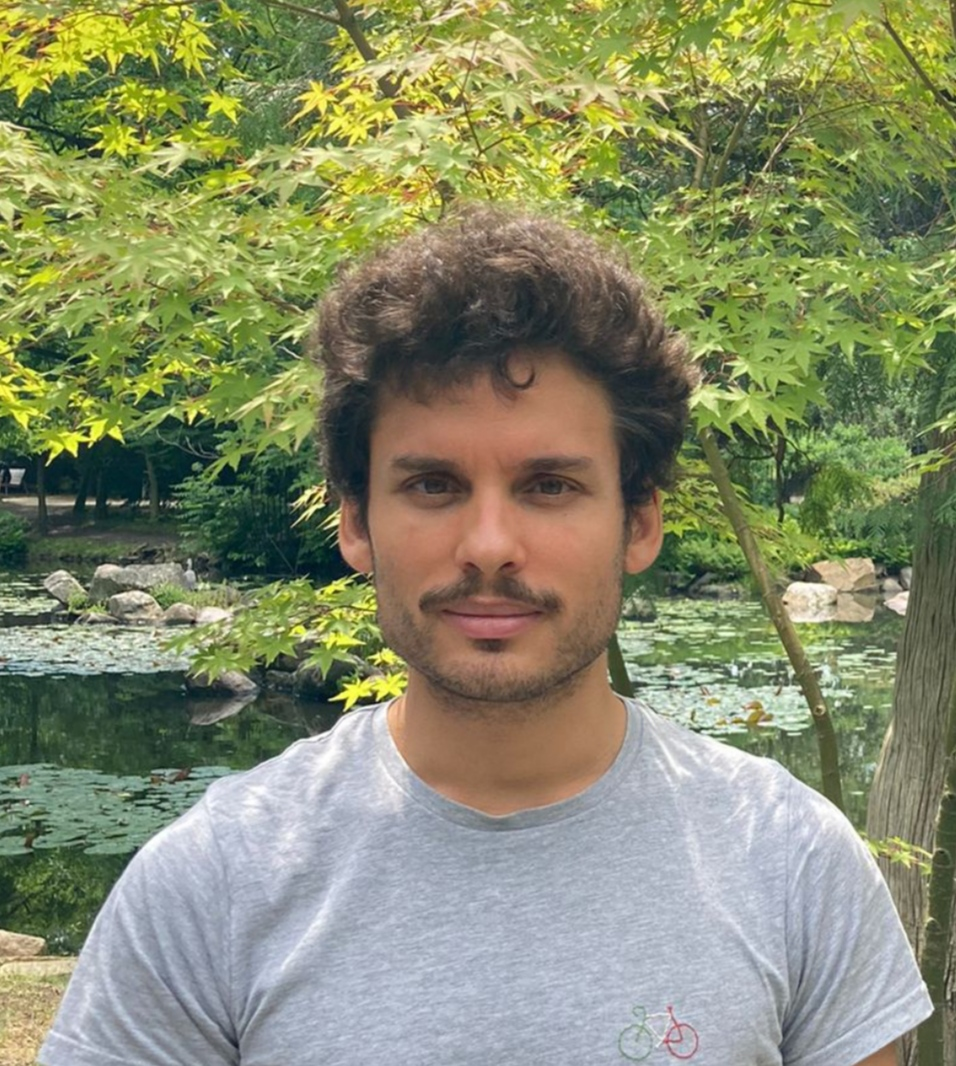
\includegraphics[height=2.4cm]{figures/mathurin.jpg}\hfill%
    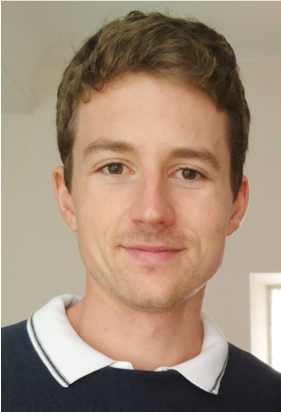
\includegraphics[height=2.4cm]{figures/quentin.png}\hfill%
    
\includegraphics[height=2.4cm]{figures/jonas.jpg}\hfill\null
  \end{center}

  Co-authored with Mathurin Massias, Quentin Bertrand, and Jonas Wallin.

\end{frame}

\begin{frame}[c]
  \frametitle{Motivation}

  \begin{itemize}[<+->]
    \item SLOPE has many appealing properties but the best algorithms for solving SLOPE are slow
          (relative to the lasso)
    \item Lasso solvers are fast because they use coordinate descent
    \item Unfortunately cannot use basic coordinate descent for SLOPE
  \end{itemize}
\end{frame}

\begin{frame}
  \frametitle{Coordinate Descent}

  \begin{columns}[c]
    \begin{column}{0.35\textwidth}
      \begin{exampleblock}{Simple Method!}
        At each iteration, update a single coordinate (coefficient).
      \end{exampleblock}
    \end{column}
    \begin{column}{0.55\textwidth}
      \begin{figure}[htpb]
        \centering
        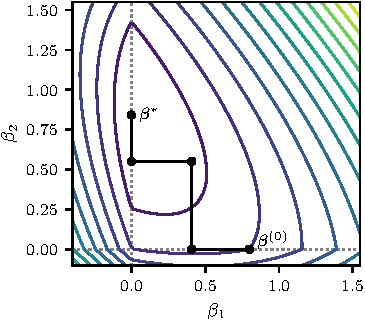
\includegraphics[]{figures/paper5-cd.pdf}
        \caption{%
          A basic example of coordinate descent in two dimensions
        }
      \end{figure}
    \end{column}
  \end{columns}
\end{frame}

\begin{frame}
  \frametitle{Coordinate Descent Performance}
  Performs (surprisingly) well!

  \medskip

  \begin{figure}[htpb]
    \centering
    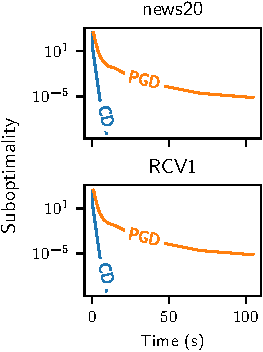
\includegraphics[]{figures/paper5-cd-vs-pgd.pdf}
    \caption{%
      Coordinate descent versus proximal gradient descent for the lasso.
    }
  \end{figure}
\end{frame}

\begin{frame}
  \frametitle{Coordinate Descent and Separability}
  \begin{columns}[T]
    \begin{column}{0.39\textwidth}
      \only<1->{%
        Cannot use basic coordinate descent for SLOPE since the
        sorted \(\ell_1\) norm is \alert{inseparable}:
        \[
          h(\vec{\beta}) = \sum_{j=1}^p \lambda_j |\beta_{(j)}|.
        \]
      }

      \medskip

      \only<2->{%
        But if we could fix the clusters, we have separability!
      }

      \medskip

      \only<3->{%
        \begin{exampleblock}{Idea}
          Alternate between gradient descent
          and coordinate descent \alert{on the clusters}.
        \end{exampleblock}
      }

    \end{column}
    \begin{column}{0.51\textwidth}
      \only<1->{%
        \begin{figure}[htpb]
          \centering
          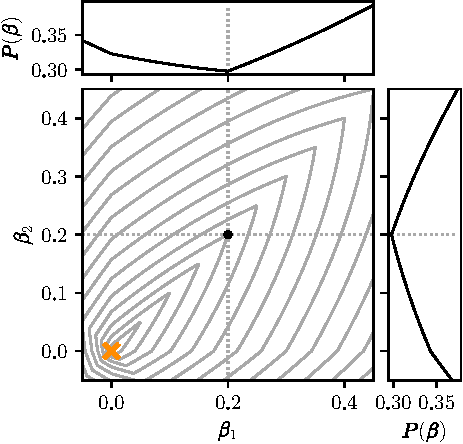
\includegraphics[width=\textwidth]{figures/paper5-naive-cd-stuck.pdf}
          \caption{A \emph{naive} coordinate descent algorithm cannot advance from the
            current iterate (\ding{108}) to reach the optimum ({\color{orange}\ding{54}}).}
        \end{figure}
      }
    \end{column}
  \end{columns}

\end{frame}

\begin{frame}[c]
  \frametitle{Hybrid Algorithm}

  \begin{itemize}
    \item Every \(v\)th iteration, take a full proximal gradient step. This allows clusters to split
          (or merge).
    \item At all other iterations, take coordinate descent steps on the clusters.
  \end{itemize}

  \pause

  \begin{figure}[htpb]
    \centering
    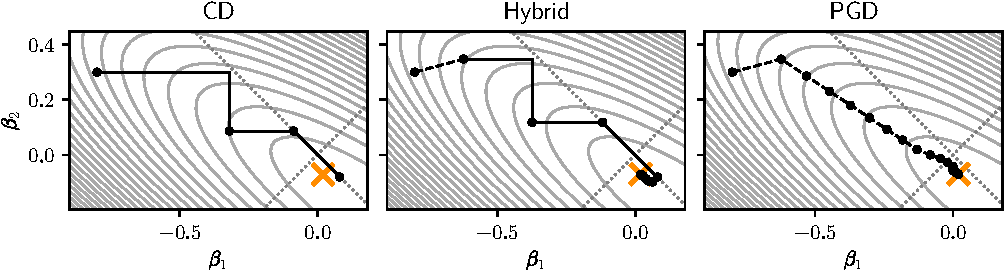
\includegraphics[width=\textwidth]{figures/paper5-illustration_solvers.pdf}
    \caption{%
      Our algorithm (hybrid) is a combination of CD and PGD.
    }
  \end{figure}
\end{frame}

\begin{frame}
  \frametitle{Experiments: Simulated Data}

  \begin{figure}[htpb]
    \centering
    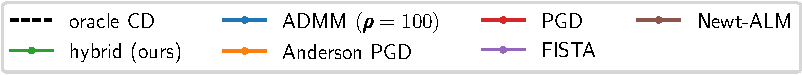
\includegraphics[scale=0.5]{figures/paper5-simulated-legend.pdf}
    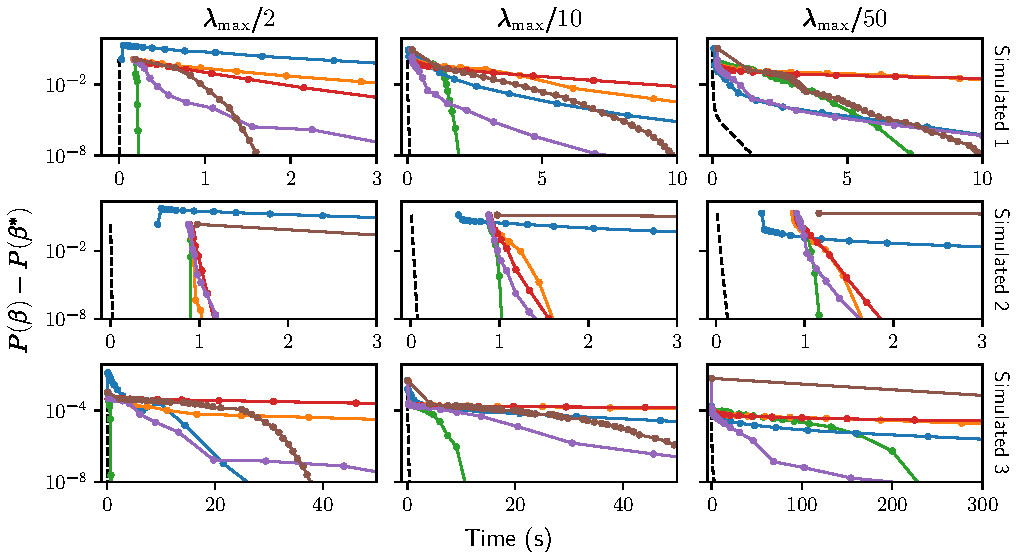
\includegraphics[scale=0.55]{figures/paper5-simulated.pdf}
    \caption{%
      Benchmarks on simulated data. Scenario 1: \(n = 200\) and \(p = 20\,000\),
      \(X\). Scenario 2: \(n = 20\,000\) and \(p = 200\). Scenario 3: \(n = 200\),
      \(p = 200\,000\), and sparse \(X\).
    }
  \end{figure}
\end{frame}

\begin{frame}[c]
  \frametitle{Summary}

  \begin{exampleblock}{Contributions}
    \begin{itemize}
      \item A hybrid algorithm for SLOPE that brings the speed of coordinate descent to SLOPE
      \item Faster than existing methods
      \item Implemented in Python package
            \texttt{sortedl1}\footnote{\url{https://pypi.org/project/sortedl1/}}
    \end{itemize}
  \end{exampleblock}

  \pause

  \begin{alertblock}{Limitations}
    \begin{itemize}
      \item Somewhat tricky to implement
      \item Not quite as fast as coordinate descent solvers for the lasso
    \end{itemize}
  \end{alertblock}
\end{frame}

\section{The Lasso and Ridge Regression Yield Biased Estimates of Imbalanced Binary Features (Paper~VI)}

\begin{frame}[c]
  \frametitle{The Lasso and Ridge Regression Yield Biased Estimates of Imbalanced Binary Features}

  Not yet published, but will be soon\texttrademark

  \bigskip

  Co-authored with Jonas.
\end{frame}

\begin{frame}[c]
  \frametitle{Motivation}

  \begin{itemize}[<+->]
    \item Most regularized methods are scale-sensitive, so have to normalize.
    \item Straightforward normalization when everything is normal, but what about features that have
          other distributions (binary features)?
    \item No literature on the effects of different normalization strategies
  \end{itemize}
\end{frame}

\begin{frame}[c]
  \frametitle{The Elastic Net}

  % Linear regression plus a combination of the \(\ell_1\) and \(\ell_2\) penalties:
  % \begin{equation*}
  %   (\hat{\beta}_0, \hat{\vec{\beta}}) = \argmin_{\beta_0 \in \mathbb{R},\beta \in \mathbb{R}^p} \left( \frac{1}{2} \lVert \vec y - \beta_0 - \mat{X}\vec{\beta} \rVert^2_2  + \lambda_1 \lVert \vec\beta \rVert_1 + \frac{\lambda_2}{2}\lVert \vec \beta \rVert_2^2\right).
  % \end{equation*}
  \begin{equation*}
    \vec{\beta}^* = \operatorname*{minimize}_{\beta \in \mathbb{R}^p} \bigg( \frac{1}{2} \lVert \vec y - \mat{X}\vec{\beta} \rVert^2_2  + \underbrace{\lambda_1 \lVert \vec\beta \rVert_1}_\text{lasso} + \underbrace{\frac{\lambda_2}{2}\lVert \vec \beta \rVert_2^2}_\text{ridge}\bigg)
  \end{equation*}

  \pause

  \begin{figure}
    \centering
    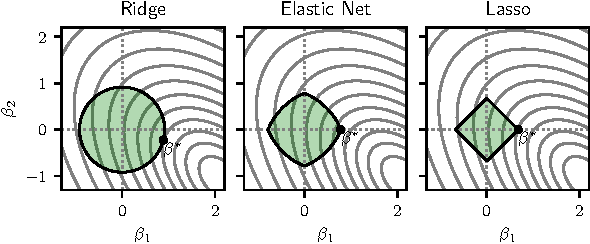
\includegraphics[width=0.85\textwidth]{figures/paper6-elasticnet-balls.pdf}
    \caption{%
      The elastic net penalty is a combination of the lasso and ridge penalties. Here shown as a constrained problem.
    }
  \end{figure}
\end{frame}

\begin{frame}[c]
  \frametitle{Sensitivity to Scale}

  Lasso and ridge penalties are \textbf{norms}---feature scales matter!

  \pause

  \begin{exampleblock}{Example}
    Assume
    \[
      \mat{X} \sim \operatorname{Normal}\left(\begin{bmatrix}0 \\ 0\end{bmatrix}, \begin{bmatrix} 4 & 0 \\ 0 & 1\end{bmatrix}\right), \qquad \vec{\beta}^* = \begin{bmatrix} \frac{1}{2} \\ 1 \end{bmatrix}.
    \]

    \medskip\pause

    \begin{table}
      \begin{tabular}{lcc}
        \toprule
        Model & \(\hat{\vec{\beta}}\)                                  & \(\hat{\vec{\beta}}_\text{std}\)                             \\
        \midrule
        OLS   & \(\begin{bmatrix} 0.50 & 1.00\end{bmatrix}^\intercal\) & \(\begin{bmatrix}1.00 & 1.00\end{bmatrix}^\intercal\) \pause \\
        Lasso & \(\begin{bmatrix} 0.38 & 0.50\end{bmatrix}^\intercal\) & \(\begin{bmatrix}0.74 & 0.50\end{bmatrix}^\intercal\) \pause \\
        Ridge & \(\begin{bmatrix} 0.37 & 0.41\end{bmatrix}^\intercal\) & \(\begin{bmatrix}0.74 & 0.41\end{bmatrix}^\intercal\)        \\
        \bottomrule
      \end{tabular}
    \end{table}
  \end{exampleblock}

  \pause

  \alert{Large} scale means \alert{less} penalization because the size of \(\beta_j\) can be smaller for an equivalent effect (on \(\vec{y}\)).

\end{frame}

\begin{frame}[c]
  \frametitle{Normalization}

  \begin{itemize}[<+->]
    \item Scale sensitivity can be mitigated by normalizing the features.
    \item Let \(\tilde{\mat X}\) be the normalized feature matrix, with elements
          \[
            \tilde{x}_{ij} = \frac{x_{ij} - c_{j}}{s_j}.
          \]
    \item After fitting, we transform the coefficients back to their original scale via
          \[
            \hat\beta_j = \frac{\hat\beta^{(n)}_j}{s_j} \quad\text{for}\quad j = 1,2,\dots,p.
          \]
  \end{itemize}

  % \bigskip\pause
  % \begin{block}{Ambiguous Nomenclature}
  %   \begin{itemize}
  %     \item Some refer to this as \emph{standardization} (which we dedicate for the mean--standard deviation combo).
  %     \item Some take normalization to mean \alert{sample-wise} normalization.
  %     \item Some take normalization to mean scaling with a \alert{norm}.
  %     \item Some refer to this (centering and scaling) as \alert{scaling}.
  %   \end{itemize}
  % \end{block}
\end{frame}

\begin{frame}[c]
  \begin{table}[hbt]
    \centering
    \caption{Common ways to normalize \(\mat{X}\)}
    \begin{tabular}{lll}
      \toprule
      Normalization    & Centering (\(c_{j}\))              & Scaling (\(s_j\))                                         \\
      \midrule
      Standardization  & \(\frac{1}{n}\sum_{i=1}^n x_{ij}\) & \(\sqrt{\frac{1}{n}\sum_{i=1}^n (x_{ij} - \bar{x}_j)^2}\) \\
      \addlinespace
      Min--Max         & \(\min_i(x_{ij})\)                 & \(\max_i(x_{ij}) - \min_i(x_{ij})\)                       \\
      \addlinespace
      Unit Vector (L2) & 0                                  & \(\sqrt{\sum_{i=1}^n x_{ij}^2}\)                          \\
      \addlinespace
      Max--Abs         & 0                                  & \(\max_i(|x_{ij}|)\)                                      \\
      \addlinespace
      Adaptive Lasso   & 0                                  & \(\beta_j^\text{OLS}\)                                    \\
      \bottomrule
    \end{tabular}
  \end{table}
\end{frame}

\begin{frame}[c]
  \frametitle{The Type of Normalization Matters}

  \begin{figure}[htpb]
    \centering
    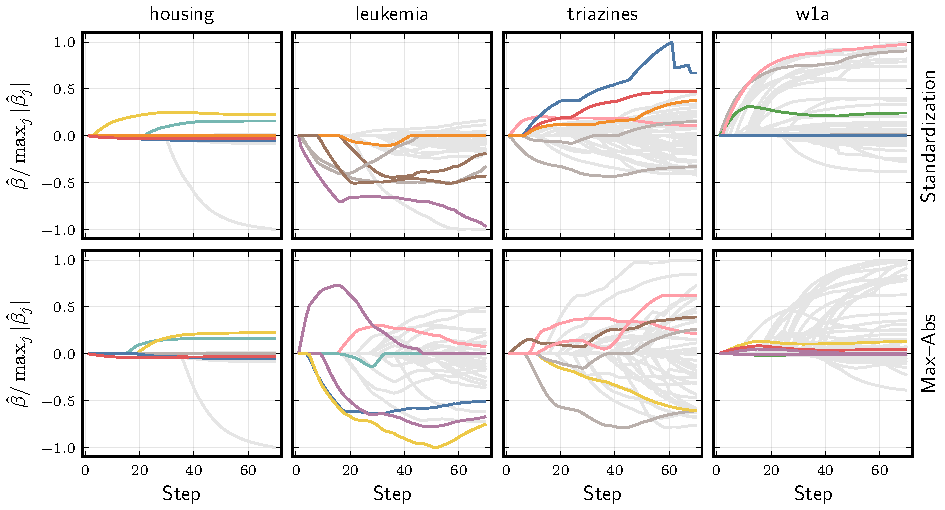
\includegraphics[width=\textwidth]{figures/paper6-realdata_paths.pdf}
    \caption{%
      Lasso paths under two different types of normalization (standardization and max--abs normalization). The union of the first five features selected in any of the schemes are colored.
    }
  \end{figure}

\end{frame}

\begin{frame}[c]
  \frametitle{Binary Features}

  \begin{columns}
    \begin{column}{0.45\textwidth}

      For binary features (values 0 and 1 only), we have for the noiseless case
      \[
        \hat{\beta}_j =
        % \frac{\operatorname{S}_{\lambda_1}(\tilde{\vec{x}}^\intercal \vec{y})}{s_j\left(\tilde{\vec{x}}_j^\intercal \tilde{\vec{x}}_j + \lambda_2\right)}
        % =
        \frac{\operatorname{S}_{\lambda_1}\left(\frac{\beta_j^* n \alert{(q - q^2)}}{s_j}\right)}{s_j\left(\frac{n\alert{(q - q^2)}}{s_j^2} + \lambda_2\right)}.
      \]
    \end{column}
    \begin{column}{0.45\textwidth}
      \begin{figure}[htpb]
        \centering
        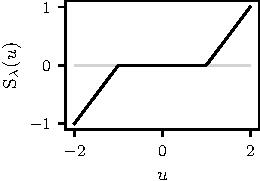
\includegraphics[]{figures/paper6-st.pdf}
        \caption{%
          Soft-thresholding
        }
      \end{figure}
    \end{column}
  \end{columns}

  \pause

  \begin{itemize}[<+->]
    \item Means that the elastic net estimator depends on class balance (\(q\)).
    \item \(s_j = q - q^2\) for lasso and \(s_j = \sqrt{q-q^2}\) for ridge removes effect of \(q\).
    \item Suggests the parametrization
          \[
            s_j = (q - q^2)^\delta, \qquad \delta \geq 0.
          \]
          % \item Indicates there is no simple \(s_j\) that works for the elastic net. (Need to use weighted
          %       elastic net.)
  \end{itemize}
\end{frame}

\begin{frame}[c]
  \frametitle{Mixed Data}

  \begin{figure}[htpb]
    \centering
    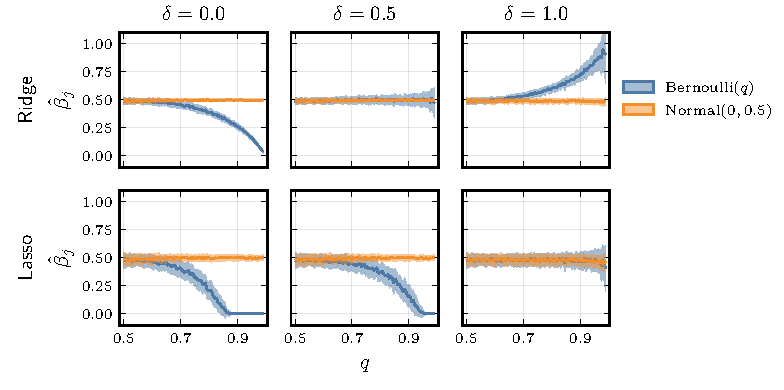
\includegraphics[width=\textwidth]{figures/paper6-mixed_data.pdf}
    \caption{%
      Comparison between lasso and ridge estimators for a data set with one binary and one quasi-normal feature.}
  \end{figure}
\end{frame}

\begin{frame}[c]
  \frametitle{Summary}
  \begin{exampleblock}{Contributions}
    \begin{itemize}
      \item As far as we know the first paper to investigate the interplay between normalization and
            regularization
      \item New scaling approach to deal with class-imbalanced binary features
      \item Discussion and suggestions for dealing with mixed data
    \end{itemize}
  \end{exampleblock}

  \pause

  \begin{alertblock}{Limitations}
    \begin{itemize}
      \item So far only theoretical results for limited cases:
            \begin{itemize}
              \item Fixed data (\(\mat{X}\)), normal noise
              \item Orthogonal features
              \item Normal and binary features
            \end{itemize}
    \end{itemize}
  \end{alertblock}
\end{frame}

\begin{frame}[c]
  \frametitle{Recap}

  \begin{itemize}[<+->]
    \item Several screening rules that improve performance for lasso and SLOPE
    \item Framework for benchmarking optimization methods
    \item Fast optimization method for SLOPE
    \item Analysis of interplay between normalization and penalization
  \end{itemize}

\end{frame}

\begin{frame}[standout]
  Thank you!
\end{frame}

\appendix

\begin{frame}[allowframebreaks]{References}
  \printbibliography[heading=none]
\end{frame}

\section{Paper I Extras}

\begin{frame}[fragile]
  \frametitle{Strong Rule Algorithm for SLOPE}
  \begin{algorithm}[H]
    \SetAlgoLined
    \KwData{\(\bm{c} \in \mathbb{R}^p\),
      \(\bm{\lambda} \in \mathbb{R}^p\), where
      \(\lambda_1 \geq \cdots \geq \lambda_p \geq 0\)}
    \(\mathcal{S}, \mathcal{B} \gets \varnothing\)\;
    \For{\(i \gets 1\) \KwTo \(p\)}{
      \(\mathcal{B} \gets \mathcal{B} \cup \{i\}\)\;
      \If{\(\sum_{j \in \mathcal{B}}\big(c_j - \lambda_j\big) \geq 0\)}{
        \(\mathcal{S} \gets \mathcal{S} \cup \mathcal{B}\)\;
        \(\mathcal{B} \gets \varnothing\)\;
      }
    }
    \Return \(\mathcal{S}\)\;
    \caption{Basic algorithm for the strong rule for SLOPE}
  \end{algorithm}
  \medskip\pause
  Set
  \[
    \bm{c} = \lvert \nabla g(\hat{\bm{\beta}})+ \bm{\lambda}^{(k-1)} - \bm{\lambda}^{(k)}\rvert_\downarrow \qquad \bm{\lambda} = \bm{\lambda}^{(k)},
  \] and run the algorithm above; the result is the predicted support for
  \(\hat{\bm{\beta}}(\bm{\lambda}^{(k)})\) (subject to a permutation).
\end{frame}

\begin{frame}[c]
  \frametitle{Results: Speed}

  \begin{figure}[htpb]
    \centering
    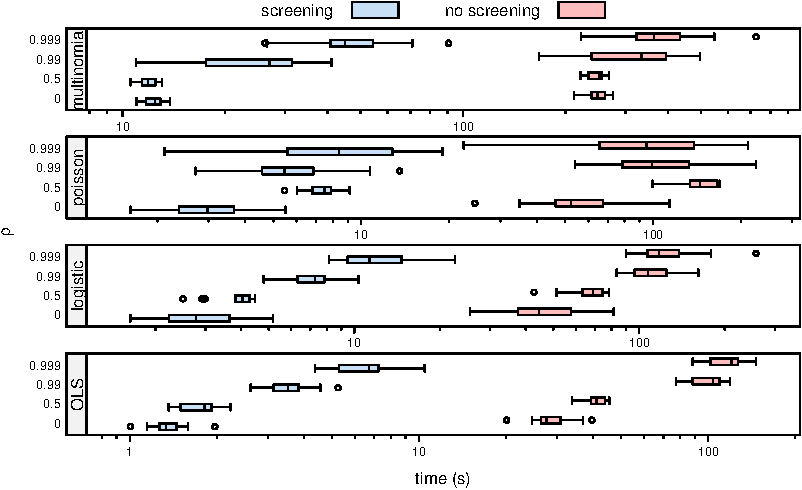
\includegraphics[width=0.95\textwidth]{figures/paper1-performance.pdf}
    \caption{%
      Time to fit a full SLOPE path with and without the strong rule
    }
  \end{figure}
\end{frame}

\section{Paper II Extras}

\begin{frame}
  \frametitle{The Dual}
  Complementary to the primal problem. For the lasso, it is
  \[
    \operatorname*{maximize}_{\vec{\theta} \in \mathbb{R}^n}
    \Bigg(
    D(\vec{\theta}; \lambda) = \frac 1 2 \vec{y}^\intercal \vec{y} -
    \frac{\lambda^2}{2} \Big\lVert \vec{\theta} - \frac{\vec{y}}{\lambda} \Big\rVert_2^2.
    \Bigg)
  \]
  \pause
  \begin{columns}
    \begin{column}{0.45\linewidth}
      \begin{block}{Duality Gap}
        Difference between the primal and dual
        objectives. Tight at the optimum (for the lasso):
        \[
          P(\vec{\beta}^*; \lambda) - D(\vec{\theta}^*; \lambda) = 0.
        \]
      \end{block}
    \end{column}
    \begin{column}{0.45\linewidth}
      \begin{figure}[htpb]
        \centering
        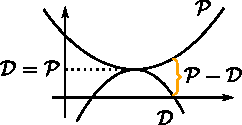
\includegraphics[]{figures/paper2-duality-gap.pdf}
      \end{figure}
    \end{column}
  \end{columns}
  \medskip

  \pause

  \begin{block}{Dual--Primal Relationship}
    The two problems are related via
    \[
      \frac{\vec{y} - \mat{X}\vec{\beta}}{\lambda} = \vec{\theta}.
    \]
  \end{block}
\end{frame}

\begin{frame}[c]
  \frametitle{Look-Ahead Screening}
  Inequality for Gaps Safe screening rule is \alert{quadratic} in \(\lambda\), which means we can find the next
  critical point easily:
  \[
    \lambda_+ = \frac{-b \pm \sqrt{b^2 - 4ac}}{2a} \quad
  \]
  where
  \[
    \begin{aligned}
      a & = \big( 1 - | \vec{x}_j^\intercal \vec{\theta}_\lambda|\big)^2 -
      \frac 12 \vec{\theta}_\lambda^\intercal \vec{\theta}_\lambda \lVert \vec{x}_j\rVert_2^2,     \\
      b & = \big(\vec{\theta}_\lambda^\intercal \vec{y} - \lVert \vec{\beta}_\lambda \rVert_1\big)
      \lVert \bm{x}_j \rVert_2^2,                                                                  \\
      c & = - \frac 12 \lVert \bm{y} - \bm{X\beta}_\lambda\rVert_2^2
      \lVert \bm{x}_j\rVert_2^2.                                                                   \\
    \end{aligned}
  \]

  \medskip\pause

  Allows us to screen predictors for \textbf{all} upcoming steps
\end{frame}

\section{Paper III Extras}

\begin{frame}
  \frametitle{Warm Starts}
  The availability of the Hessian inverse enables a better warm start:
  \[
    \hat\beta(\lambda_{k+1})_\mathcal{A} =
    \hat\beta(\lambda_k)_\mathcal{A} +
    (\lambda_k - \lambda_{k+1}) \big({X_\mathcal{A}}^T{X_\mathcal{A}}\big)^{-1}
    \sign\big(\hat\beta(\lambda_k)_\mathcal{A}\big)
  \]

  \pause

  \begin{figure}
    \centering
    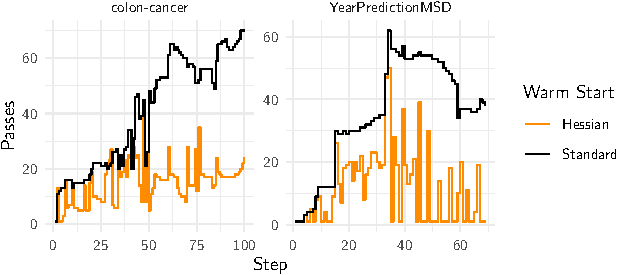
\includegraphics{figures/paper3-warm-starts}
    \caption{Number of passes of coordinate descent for two datasets
      using either Hessian warm
      starts or standard warm starts.}
  \end{figure}
\end{frame}

\begin{frame}
  \frametitle{Updating the Hessian}
  Computing the Hessian and its inverse naively is expensive:
  \(\mathcal{O}(|\mathcal{A}|^3 + |\mathcal{A}|^2n)\)

  \medskip\pause

  Fortunately, we can sweep columns of the Hessian and inverse in our out, yielding
  complexity
  \begin{itemize}
    \item \(\mathcal{O}(|\mathcal{D}|^2n + n|\mathcal{D}||\mathcal{E}| +
          |\mathcal{D}^2||\mathcal{E}| + |\mathcal{D}|^3)\) when
          augmenting the Hessian and
    \item \(\mathcal{O}(|\mathcal{C}|^3 + |\mathcal{C}|^2|\mathcal{E}| +
          |\mathcal{C}||\mathcal{E}|^2)\) when reducing it,
  \end{itemize}
  where
  \begin{itemize}
    \item \(\mathcal{C} = \mathcal{A}_{k-1} \setminus \mathcal{A}_k\)
          (to-be deactivated)
    \item \(\mathcal{D} = \mathcal{A}_k \setminus \mathcal{A}_{k-1}\)
          (to-be activated)
    \item \(\mathcal{E} = \mathcal{A}_k \cap \mathcal{A}_{k-1}\)
          (still activate)
  \end{itemize}
\end{frame}

\section{Paper V Extras}

\begin{frame}
  \frametitle{How Do We Minimize Over One Cluster?}

  \begin{columns}
    \begin{column}{0.45\textwidth}
      The optimality condition, using the directional derivative, is
      \[
        \forall \delta \in \{-1, 1\}, \quad G'(z; \delta) \geq 0,
      \]
      with
      \[
        \begin{multlined}
          G'(z; \delta)  \\= \delta \sum_{j \in \mathcal{C}_k} X_{:j}^\top(X\beta(z) - y) \\
          + H'(z; \delta).
        \end{multlined}
      \]
    \end{column}
    \begin{column}{0.45\textwidth}
      \begin{figure}
        \centering
        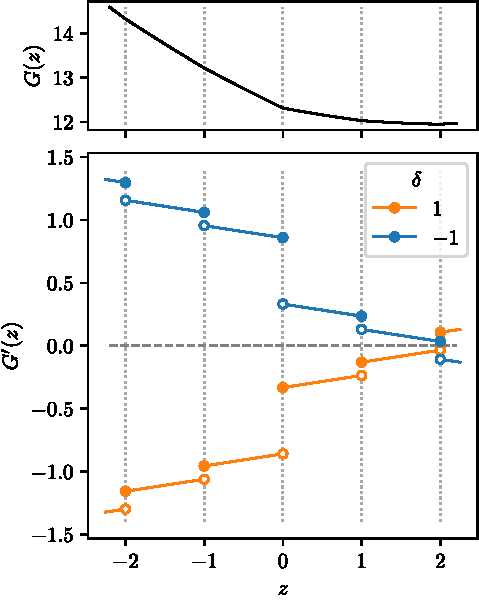
\includegraphics[width=0.9\textwidth]{figures/paper5-directional-derivative.pdf}
        \caption{%
        \(G\) and its directional derivative \(G'( \cdot ; \delta)\) for
        an example with \(\beta = [-3, 1, 3, 2]^T\), \(k = 1\), and consequently
        \(c^{\setminus k} = \{1, 2\}\).
        }
      \end{figure}
    \end{column}
  \end{columns}
\end{frame}

\begin{frame}
  \frametitle{The SLOPE Thresholding Operator}

  \begin{figure}[htpb]
    \centering
    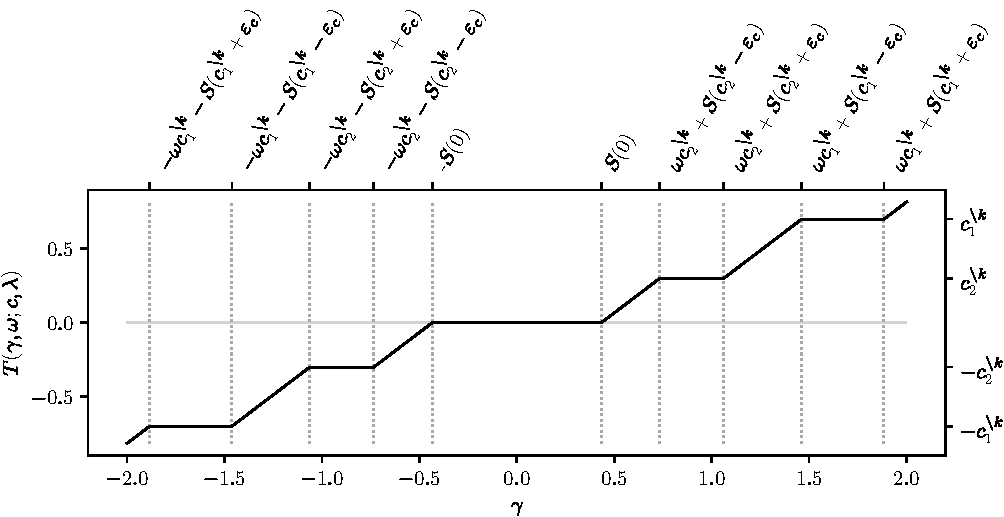
\includegraphics[width=\textwidth]{figures/paper5-slope-thresholding.pdf}
    \caption{%
      The SLOPE Thresholding Operator
    }
  \end{figure}
\end{frame}

\begin{frame}
  \frametitle{Experiments: Real Data}

  \begin{figure}
    \centering
    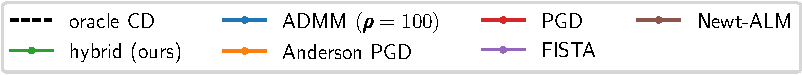
\includegraphics[scale=0.55]{figures/paper5-real_legend.pdf}
    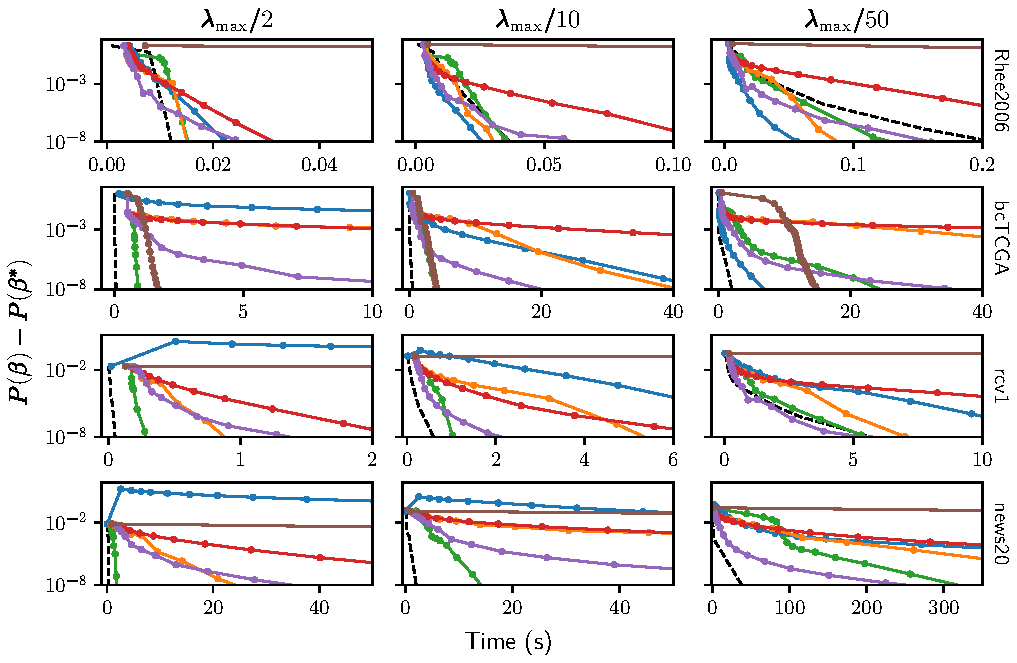
\includegraphics[scale=0.55]{figures/paper5-real.pdf}
    \caption{%
      Benchmarks on real data
    }
  \end{figure}
\end{frame}

\section{Paper VI Extras}

\begin{frame}[c]
  \frametitle{Probability of Selection}

  Since \(\mat{X}\) is fixed and \(\vec{\varepsilon}\) is normal, it is straightforward to
  compute the probability of selection:
  \[
    \Pr(\hat{\beta}_j \neq 0) = \Phi\left(\frac{\mu - \lambda_1}{\sigma}\right) + \Phi\left(\frac{- \mu -\lambda_1}{\sigma}\right).
  \]

  \begin{figure}[htpb]
    \centering
    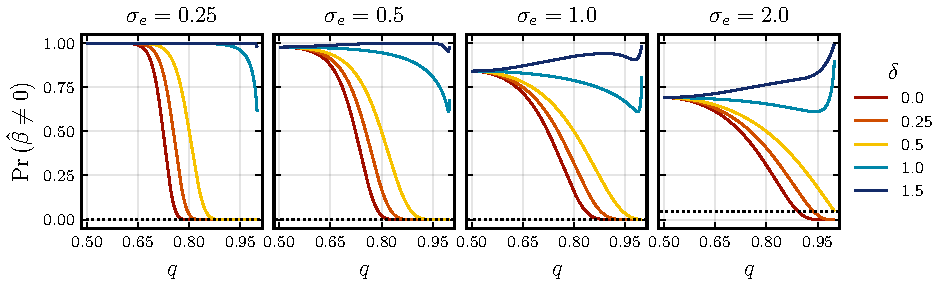
\includegraphics[width=\textwidth]{figures/paper6-selection_probability.pdf}
    \caption{%
      Probability that the elastic net selects a feature across different noise levels \((\sigma_\varepsilon)\), types of normalization (\(\delta\)), and class balance (\(q\)).
      The dashed line is asymptotic behavior for \(\delta = 1/2\).
    }
  \end{figure}
\end{frame}

\begin{frame}[c]
  \frametitle{Asymptotic Results for Bias and Variance}

  \begin{theorem}
    If \(\bm{x}_j\) is a binary feature with class balance \(q \in (0, 1)\) and \(\lambda_1,\lambda_2 \in (0,\infty)\), \(\sigma_\varepsilon > 0\), and \(s_j = (q - q^2)^{\delta}\), \(\delta \geq 0\), then
    \[
      \lim_{q \rightarrow 1^+} \E \hat{\beta}_j =
      \begin{cases}
        0                                                                                                  & \text{if } 0 \leq \delta < \frac{1}{2}, \\
        \frac{2n \beta_j^*}{n + \lambda_2} \Phi\left(-\frac{\lambda_1}{\sigma_\varepsilon \sqrt{n}}\right) & \text{if } \delta = \frac{1}{2},        \\
        \beta^*_j                                                                                          & \text{if } \delta \geq \frac{1}{2}.
      \end{cases}
    \]
    \pause and
    \[
      \lim_{q \rightarrow 1^+} \var \hat{\beta}_j =
      \begin{cases}
        0      & \text{if } 0 \leq \delta < \frac{1}{2}, \\
        \infty & \text{if } \delta \geq \frac{1}{2}.
      \end{cases}
    \]
  \end{theorem}

\end{frame}

\begin{frame}[c]
  \frametitle{A Bias--Variance Tradeoff}

  \begin{figure}
    \centering
    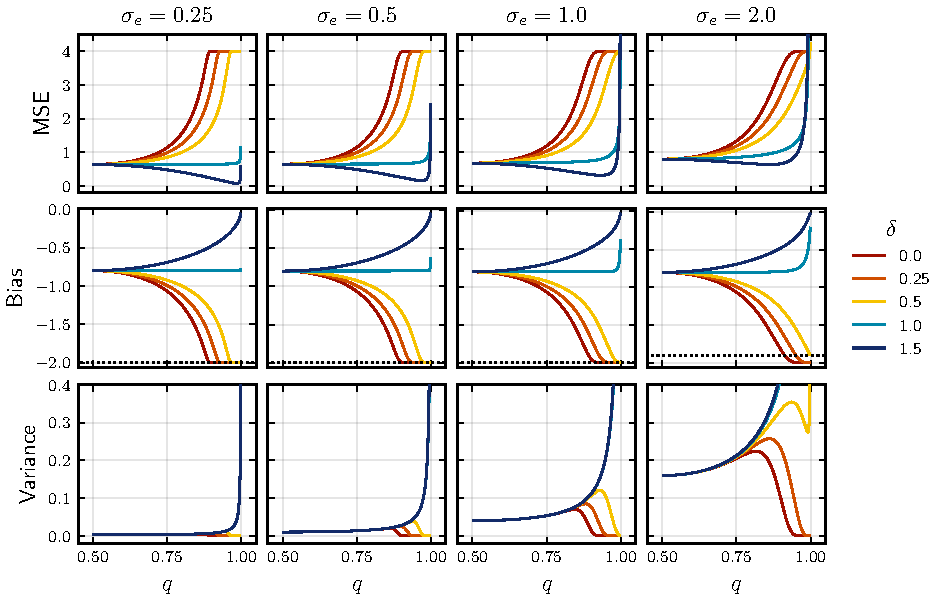
\includegraphics[width=0.94\textwidth]{figures/paper6-bias-var-onedim.pdf}
    \caption{%
      Bias, variance, and mean-squared error for a one-dimensional lasso problem. Theoretical result for orthogonal features. Dotted line is asymptotic result or \(\delta = 1/2\).
    }
  \end{figure}

\end{frame}

\begin{frame}[c]
  \frametitle{Multiple Features: Power, FDR, and NMSE}

  Lasso example with 10 true signals and varying \(q\) and \(p\).

  \begin{figure}[htpb]
    \centering
    \subcaptionbox{%
      Power in the sense of detecting all the true signals. Constant \(p\).
    }{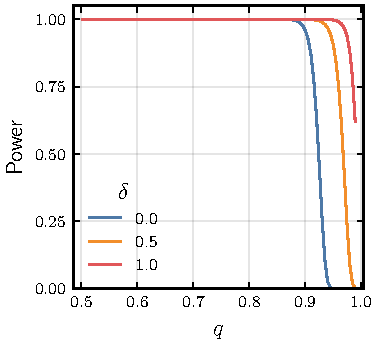
\includegraphics[width=0.35\textwidth]{figures/paper6-power.pdf}}\hfill\pause%
    \subcaptionbox{%
      False discovery rate (FDR) and normalized mean-squared error (NMSE).
    }{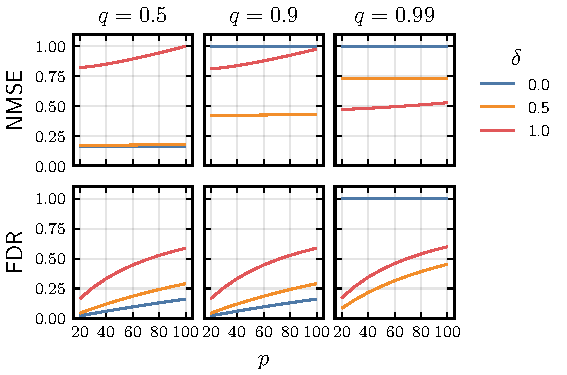
\includegraphics[width=0.55\textwidth]{figures/paper6-fdr_mse.pdf}}
    \caption{%
      Mean squared error (MSE), false discovery rate (FDR), and power.
    }
  \end{figure}
\end{frame}

\begin{frame}[c]
  \frametitle{Hyperparameter Optimization}

  \textbf{Idea:} The choice of \(\delta\) affects the model, so let's optimize over it.

  \begin{figure}[htpb]
    \centering
    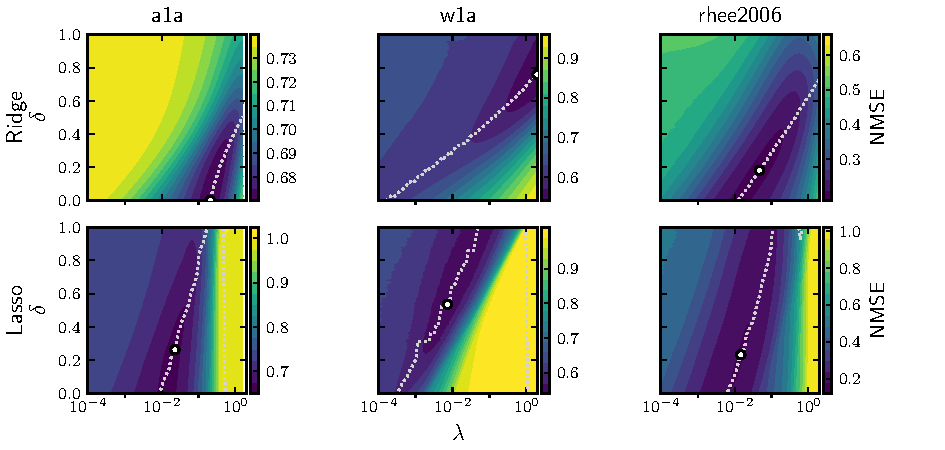
\includegraphics[width=\textwidth]{figures/paper6-hyperopt_surfaces.pdf}
    \caption{%
      Contour plots of hold-out (validation set) error across a grid of \(\delta\) and \(\lambda\) values for the
      lasso and ridge.
    }
  \end{figure}
\end{frame}

\end{document}

